\documentclass[a4paper]{article}
\usepackage[T1]{fontenc}
\usepackage{amsmath}
\usepackage{hyperref}
\usepackage{amsthm}
\usepackage{amssymb}
\usepackage{float}
\usepackage[utf8]{inputenc}
\usepackage[italian]{babel}
\usepackage{graphicx} 
\graphicspath{{figures/}}
\newcommand{\lcc}{\textit{largest connected component}}
\begin{document}

\author{
	Lorenzo Dentis, \textit{lorenzo.dentis@edu.unito.it}\\
	Roberto Casale, \textit{roberto.casale719@edu.unito.it}\\
	Alessandro Nocera, \textit{alessandro.nocera@edu.unito.it}
}
\title{Relazione progetto Network Science}
\maketitle

\tableofcontents

\section{appunti da scrivere ordinatamente nelle sezioni}
%TODO: Citare
"We show that social relationships can explain about 10\% to 30\% of all human movement, while periodic behavior explains 50\% to 70\%"

Clustering: Per il discorso della triadic clousure ci aspettiamo questo valore molto alto, ma nel nostra caso è "0,17" quindi le persone che partecipano allo studio non è detto che sono "amici" tra di loro.
Es. io partecipo a questo studio ma i miei amici (per cui vale la triadic closure) è improbabile ch epartecipino.

Largest component size: Il risultato ottenuto è molto alto (il 96\% dei nodi fa parte della gigant component), c'è un enorme gigant component e tutti gli altri sottografi sono formati da 3/4 nodi. ipotesi:potrebbero essere tutti vicini geograficamente oppure la "classe" dei nodi, oppure per via degli hub presenti oppure ci sono luoghi molto trafficati.
Guardando i degree di tutti i nodi della solo largest component notiamo una presenza di super hub (1000+,800,ecc..)

Degree correlation: tendenza a nodi con un certo degree a connettersi a nodi con un degree simili o uguale
ci aspettiamo che sia assortativa perchè abbiamo una grossa gigant component e una core perifery structure

le cose delle super hub era sbagliata , potrebbero essere delle comunities. degree di 1000 su 58000 nodi non è alto

l'assortativity è neutra perchè ci sono comunities


potrebbe essere bilanciata dagli altri nodi con degree basso


Comunities:set di nodi molto interconnessi
ci aspettiamo tante comunità
abbiamo 218 comunità (tante) quindi non abbiamo dei super hub, ne abbiamo solo 2

\section{Analisi}
\subsection{Dataset}
Il dataset che abbiamo analizzato è il seguente: \href{http://snap.stanford.edu/data/loc-brightkite.html}{ Friendship and Mobility: User Movement in Location-Based Social Networks }(E. Cho, S. A. Myers, J. Leskovec.).\\
Contiene dati anonimi estratti dal social-network \textit{Brighthike}, un social basato sulla posizione.
In qualsiasi momento un utente ha la possibilità di condividere la sua posizione e cercare altre persone geograficamente vicine che fanno uso di quel social, c'è anche la possibilità di segnalare che si è stati in un posto preciso ad una data ora.
Il dataset preso in esame è una restrizione di questi dati secondo 3 filtri:
\begin{itemize}
	\item Temporale: Sono presenti solo risultati raccolti tra Apr. 2008 e Ott. 2010.
	\item Spaziale: In generale tutte le coordinate si riferiscono a luoghi interni agli USA, ci sono però delle rare eccezioni, come mostrato in figura \ref{FIG:posizione_generica}
		\begin{figure}[!ht]
			\centering
			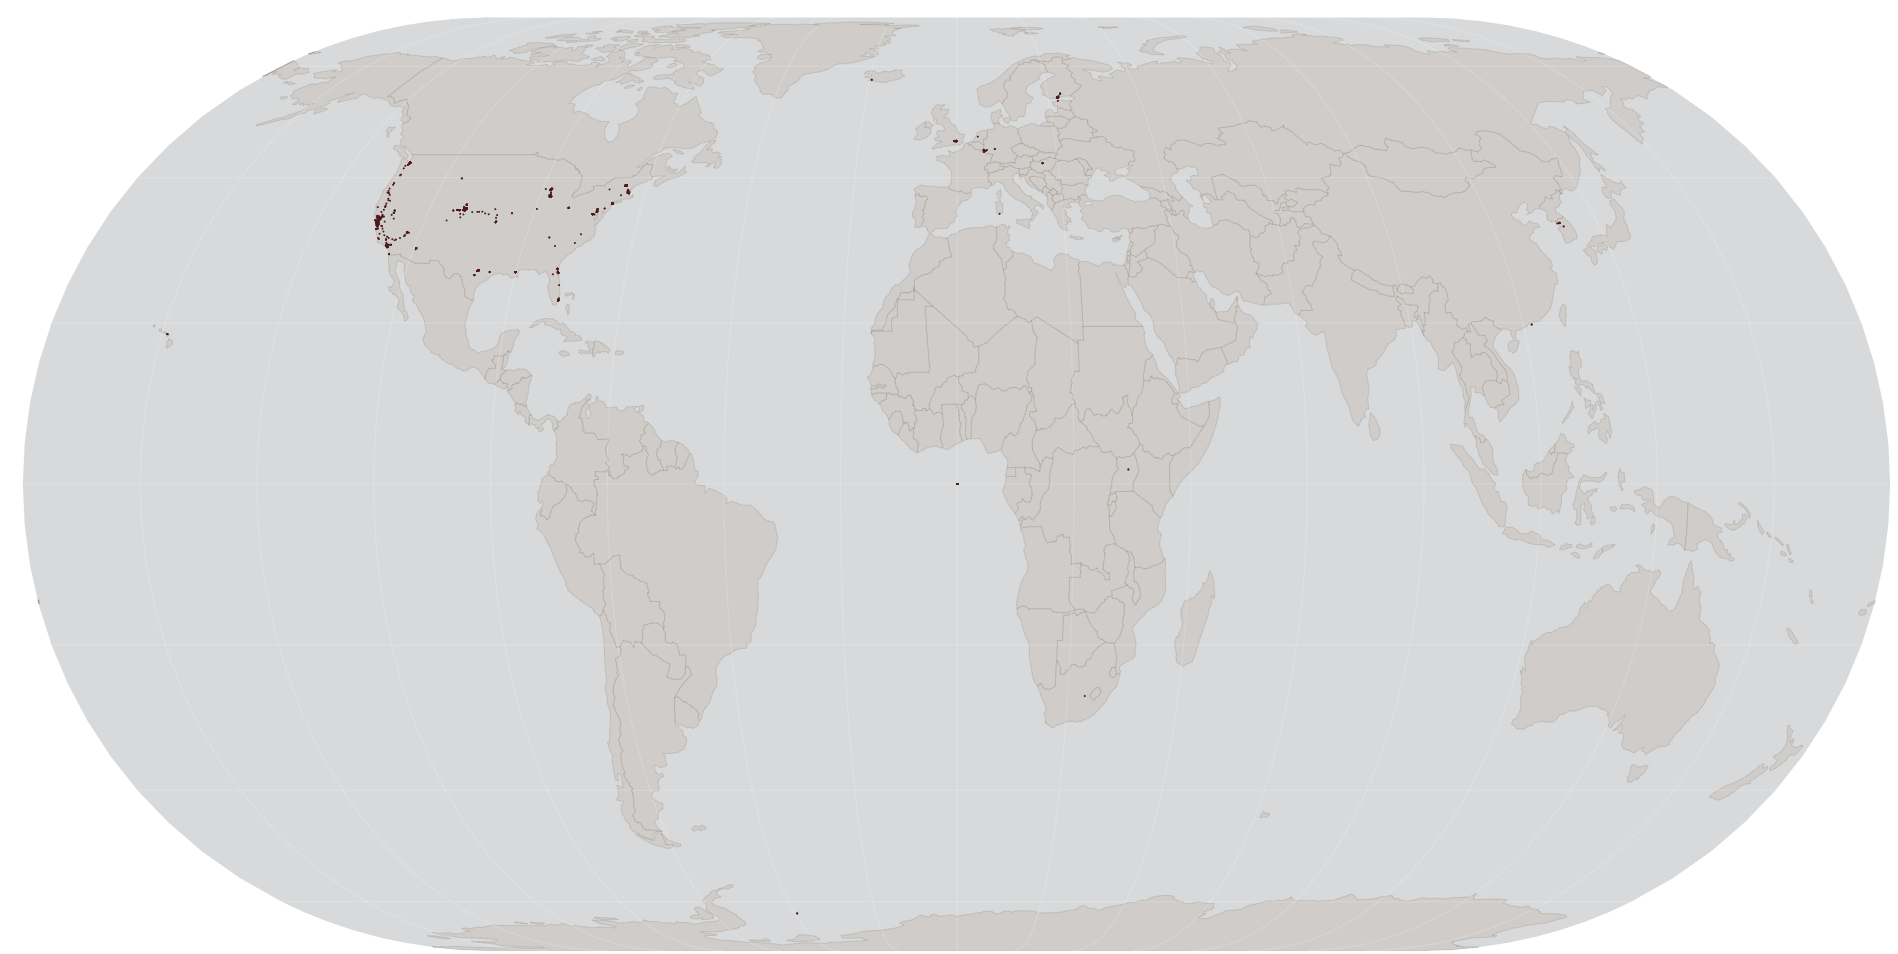
\includegraphics[width=\linewidth]{posizione_generica}
			\caption{mappa con coordinate}
			\label{FIG:posizione_generica}
		\end{figure}
		Non vi è una spiegazione ma si possono fare delle ipotesi, il social potrebbe essersi diffuso solo in America e negli Stati Europei molto meno.
		L'ipotesi che ci sentiamo di avanzare è che i dati raccolti siano solo di utenti Americani ed i luoghi \textit{outliers} siano luoghi in cui l'utente ha viaggiato (molti di questi sono luoghi turistici)
	\item Sociale: Sono stati mantenuti solo gli archi che indicavano incontri, quindi se un nodo ha effettuato \textit{check-in} in un dato luogo ma nessuno era presente il dato è stato eliminato.
		Questo fa si che sia possibile avere archi duplicati (due persone che si incontrano diverse volte in luoghi diversi o momenti diversi) ed archi monodirezionali, ad esempio un utente potrebbe aver guardato se ci fosse qualcuno nelle vicinanze e poi non averlo contattato.\\
		Tutti gli archi monodirezionali sono stati trasformati in bidirezionali perchè per lo scopo della ricerca era importante registrare gli incontri, che questi fossero o meno rappresentativi di una interazione sociale
\end{itemize}

\subsection{Dataset e approssimazioni}
Il dataset è composto da $58228$ nodi e $214078$ archi, rappresentanti un incontro tra due nodi, ciò lo rende a volte intrattabile ma fornisce anche la possibilità di effettuare operazioni di approssimazione e vedere come queste si comportano rispetto a differenti misure.
L'operazione di approssimazione più efficace che abbiamo trovato è stata la scelta di ridurre il dataset ai soli dati raccolti in un anno (2009), ciò ha portato ad un dimezzamento dei nodi (24568 nodi e 19898 archi) rendendo possibili computazioni troppo dispendiose altrimenti.
E' stato generato anche una terzo dataset, andando a focalizzarsi sui luoghi visitati, difatti tali luoghi possono essere visti come \textit{foci} ed hanno un grosso impatto sul meccanismo di creazione degli archi.

\subsection{Distanze}
Questa è stata la prima operazione che ha richiesto una approssimazione, difatti è stato usato il grafo relativo ai dati del solo anno $2019$, dovendo cercare uno shortest path per ogni coppia di nodi l'algoritmo di \textit{path finding} verrebbe eseguito potenzialmente $n*(n-1)$, cioè $3^.363^.942^.000$. ($n$ è il numero di nodi facende parte della \textit{largest connected component}, brevemente \textit{lcc}.
Il grafo non è completamente connesso, ma un rapido controllo ha indentificato che il 96\% dei nodi si trovavano nella \lcc, quindi analizzare il grafo completo è computazionalmente troppo intensivo.


Il calcolo delle distanze sul dataset ridotto ha fornito misure in linea con quanto ci si aspettava, il diametro (il più lungo shortest path) è $16$ mentre la media è molto bassa, $1,103$. Questo valore si spiega analizzando le componenti fortemente connesse.
Vi è infatti una enorme componente connessa massimale, ma quasi tutti i nodi rimanenti sono in \textit{clusters} molto piccoli, addirittura di sole due persone. Questo abbassa tantissimo la media perciò risulta molto più interessante studiare l'\textit{average\_shortest\_path} della sola componente massimale.\\
Questi risulta essere $5,71$ in linea con l'esperimento effettuato da Stanley Milgram che rilevava 6 gradi di separazione tra tutte le coppie di nodi, in questa rete la \textit{small world hypothesis} è confermata. 

\subsection{Componenti connesse}
Analizzando tutte le componenti formtemente connesse ne individuiamo $547$, di seguito una lista delle prime 10 in ordine decrescente di dimensione.\\
\begin{tabular}{ | c | c | c | c | c | c | c | c | c | c | }
  \hline
  56739 & 49 & 11 & 11 & 10 & 10 & 9 & 8 & 8 & 7\\
  \hline
\end{tabular}\\
Il 96\% dei nodi fa parte della \lcc, tutte le altre componenti connesse sono formati da meno di 3/4 nodi. 
Ci sono due differenti possibilità per spiegare questo fenomeno (le due possibilità saranno analizzate meglione nella sezione CITARE LA SEZIONE STUDIO DEI FOCI): Esiste un luogo geografico dove molte persone si sono incontrate (cioè tutti gli utenti vivono in una area geografica ridotta) oppure u
%TODO: ipotesi:potrebbero essere tutti vicini geograficamente oppure la "classe" dei nodi, oppure per via degli hub presenti oppure ci sono luoghi molto trafficati, plottare 
\section{Simulazione dinamica}
\end{document}

